% --------------------------------------
% Document Class
% --------------------------------------
\documentclass[a4paper]{article}
% --------------------------------------

% --------------------------------------
% Use Package
% --------------------------------------

% french, english
\usepackage[francais]{babel}

% font, french accent
\usepackage[utf8]{inputenc} 
\usepackage[T1]{fontenc} 

% page layout
\usepackage{geometry}
\usepackage{multicol}
\setlength{\columnsep}{4cm}

% hypertext link
\usepackage[pdfpagelabels]{hyperref}

\usepackage{graphicx}
\usepackage{float}
\usepackage{verbatim}
\usepackage{fancyhdr}
\usepackage{amsmath}

\usepackage{csquotes}

% table of contents setting
\usepackage[]{titletoc}

% include pdf
\usepackage[final]{pdfpages}

% insert code
\usepackage{listings}

% define our color
\usepackage{xcolor}

\usepackage{titlesec}

% bibliographie
\usepackage[nottoc, notlof, notlot]{tocbibind}

% code color
\definecolor{ligthyellow}{RGB}{250,247,220}
\definecolor{darkblue}{RGB}{5,10,85}
\definecolor{ligthblue}{RGB}{1,147,128}
\definecolor{darkgreen}{RGB}{8,120,51}
\definecolor{darkred}{RGB}{160,0,0}
\definecolor{univ}{RGB}{177,23,119}
\definecolor{univmodif}{RGB}{148,74,120}
\definecolor{mygray}{RGB}{100,100,100}


\lstset{
    language=C++,
    captionpos=b,
    extendedchars=true,
    frame=lines,
    numbers=left,
    numberstyle=\tiny,
    numbersep=5pt,
    keepspaces=true,
    breaklines=true,
    showspaces=false,
    showstringspaces=false,
    breakatwhitespace=false,
    stepnumber=1,
    showtabs=false,
    tabsize=3,
    basicstyle=\small\ttfamily,
    backgroundcolor=\color{ligthyellow},
    keywordstyle=\color{ligthblue},
    morekeywords={include, printf, uchar},
    identifierstyle=\color{darkblue},
    commentstyle=\color{darkgreen},
    stringstyle=\color{darkred},
}


% --------------------------------------



% --------------------------------------
% Page setting
% --------------------------------------
%\pagestyle{empty}


\setcounter{secnumdepth}{3}
\setcounter{tocdepth}{2}

\makeatletter
\@addtoreset{chapter}{part}
\makeatother 

\hypersetup{         % parametrage des hyperliens
  colorlinks=true,      % colorise les liens
  breaklinks=true,      % permet les retours à la ligne pour les liens trop longs
  urlcolor= blue,       % couleur des hyperliens
  linkcolor= black,     % couleur des liens internes aux documents (index, figures, tableaux, equations,...)
  citecolor= green      % couleur des liens vers les references bibliographiques
}

% --------------------------------------


% --------------------------------------
% Table of contents setting
% --------------------------------------
\titlecontents{section}
[0pt]% left margin
{\vspace{3mm}}% up margin
{\large\contentslabel[\thecontentslabel]{15pt}}% numbered format
{\large\contentslabel{0pt}}% unnumbered format
{\dotfill\thecontentspage}% filler-page-format, e.g dots

\titlecontents{subsection}
[30pt]% left margin
{\vspace{2mm}}% up margin
{\normalfont\contentslabel[\thecontentslabel]{20pt}}% numbered format
{}% unnumbered format
{\dotfill\thecontentspage}% filler-page-format, e.g dots

\contentsfinish
% --------------------------------------


% --------------------------------------
% Information
% --------------------------------------
\title{Compte-rendu projet individuel 96 : les yeux nous trahissent ?}
\author{Auteurs : Elliot VANEGUE et Gaëtan DEFLANDRE\\
	Encadrant : Marius BILASCO, Benjamin ALLAERT et José MENNESSON\\}
% --------------------------------------



% --------------------------------------
% Begin content
% --------------------------------------
\begin{document}

  % Set language to french
  \selectlanguage{francais}
  
  % Start the page counting
  \pagenumbering{arabic}
  
  % page de garde
  \pagestyle{empty}

% adjust pading
%\setlength{\parindent}{-2mm}


\begin{center}
  \hrule
  \vspace{1cm}
  \textbf{
  {\LARGE  
    Rapport de projet individuel\\
    \vspace{0.3cm}
    Sujet 96: Les yeux nous trahissent
  }}\\
  \vspace{0.8cm}
  {\large\textit{\textcolor{mygray}{Projet de second semestre de Master Informatique}}}\\
  \vspace{0.8cm}
  \hrule

  \vspace{3cm}
  
\includegraphics[height=3.5cm]{image/logoLILLE1.jpg}
  \hfill
  
\includegraphics[height=3.5cm]{image/logoFOX.png}
  \vspace{4cm}

  \vspace{1cm}
  {\large\textbf{\textcolor{univmodif}{Janvier à Mai 2015}}}
  \vspace{2cm}
\end{center}

\begin{multicols}{2}  

    \textbf{\textcolor{univmodif}{Auteurs:}}\\
    \begin{itemize}
      \item Elliot VANEGUE
      \item Gaëtan DEFLANDRE
    \end{itemize}
    
    \textbf{\textcolor{univmodif}{Encadrants:}}
    \begin{itemize}
      \item Marius BILASCO
      \item José MENNESSON
      \item Benjamin ALLAERT
    \end{itemize}

\end{multicols}
  
  

\pagestyle{fancy}

%%%% Style des sections %%%%
%\titleformat{\section}
\titlespacing{\section}{0em}{0em}{1em}

%%%% Style des subsections %%%%
\titleformat{\subsection}
{\large\bfseries}
{\thesubsection}{1em}{}
\titlespacing{\subsection}{1.5em}{1em}{1em}

%%%% Style des subsubsections %%%%
\titleformat{\subsubsection}
{\normalfont}
{\thesubsubsection}{1em}{}
\titlespacing{\subsubsection}{2.5em}{1em}{0.3em}

%%%% Entête %%%%
\fancyhead{}
% \fancyhead[R]{\colorbox{ivi}{
%    \begin{minipage}{0.1\textwidth}
%       \textcolor{white}{\LARGE{PJE}}
%    \end{minipage}%
% }}
\fancyhead[R]{{\Large{PJI}}}
\lhead{\raisebox{17px}{\leftmark}} % Le titre de la partie courante

%%%% Pied de page %%%%%
%\fancyfoot{}
\lfoot{
\includegraphics[height=30px]{image/logoLILLE1.jpg}}
\rfoot{
\includegraphics[height=30px]{image/logoFOX.png}}
%\rfoot{\raisebox{13px}{{\thepage} /\ \pageref{LastPage}}}

  
  %\maketitle
  %\mbox{}
  
 
  
  \newpage
  \clearpage
  
  
  \section*{Remerciement}
%\addcontentsline{toc}{section}{Remerciement}

\newpage
  \section*{Résumé}
\addcontentsline{toc}{section}{Résumé}

\section*{Abstract}
\addcontentsline{toc}{section}{Abstract}

\newpage
  
  \tableofcontents
  \newpage
  \listoffigures
    
  \section{Introduction}
%\addcontentsline{toc}{section}{Introduction}

% Préambule
%Durant nos études de master informatique à l'université de Lille 1,
%nous avons l'occasion de participer à un projet proposé par une équipe de
%recherche. Cette expérience a pour but de nous faire découvrir le
%milieu de la recherche.\\
Pour nos études en master informatique, nous participons à un projet proposé par une 
équipe de recherche. Cela nous permet de décourvir le milieu de la recherche.

% Introduction
L'application sur laquelle nous travaillons permet de localiser le visage
d'un individu au travers d'un flux vidéo afin de reconnaitre sur celui-ci différente
émotion comme la fatigue ou encore l'intérêt de la personne pour différents sujets. Ce procédé
se démocratise et il est de plus en plus utilisé dans des applications dans le domaine : 
\begin{itemize}
 \item de la sécurité, ce qui permettrai de détecter des comportements inhabituel chez un individu.
 \item du loisir, pour les jeux vidéo ou encore pour une intéraction plus intuitif avec un ordinateur.
 \item de la publicité, pour que celle-ci corresponde au besoin des individu. 
\end{itemize}
\ \\
Ce type d'application utilise différentes technologies, mais celle-ci sont souvent trop intrusifs 
et demande à l'utilisateur d'utiliser du materiel assez spécifique. Or le but des algorithmes actuel
est de faire en sorte que l'utilisateur ne se rende même pas compte qu'il utilise ce type de technologie. Les applications plus 
moderne effectue des algorithmes de reconnaissance de forme, tel que l'algorithme de Viola et Jones, dans 
le but de détecter un visage à partir de simple caméra. Cela permet de mieu intégrer ces applications 
afin qu'il n'y est aucune contrainte pour l'utilisateur.\\

L'objectif de l'application sur lequel nous travaillons est de détecter les mouvements
du visage de l'utilisateur afin d'effectuer de la reconnaissance d'émotions lors d'application
du type e-learning\footnote{formation en ligne}. Ce procédé permettrai de détecter si un cours 
intéresse ou non les élèves afin de pouvoir l'améliorer. Si on voit sur une partie du cour
que de nombreux élèves ont présentés des signes de fatigue ou qu'ils n'écoutaient plus, il sera
alors possible aux enseignant de modifier cette partie.


% Contexte
\subsection{Contexte}
Pour la réalisation de ce projet, nous travaillons avec l'équipe FOX qui étudie
l'analyse du mouvement à partir de vidéos. Leurs recherches portent
sur l'extraction du comportement humain depuis les flux vidéo.  Leurs travaux sont
divisés en quatre grands domaines : le regard, qui est la partie sur laquelle nous travaillons, l'événement, l'émotion et la
reconnaissance de personnes. La grande majorité de leurs travaux sont
des applications temps réel, ce qui permet d'avoir un niveau de réactivité très élevé.\\ 

Le projet sur lequel nous travaillons est basé sur les travaux d'anciens étudiants qui se sont concentrés sur la
détection de visage et des yeux. Une première approche de la reconnaissance d'émotion sur une vidéo a été 
réalisé par les chercheurs de l'équipe, mais elle n'est pas encore optimal. Le projet est une application temps réel, 
dont les flux vidéo peuvent provenir de vidéos enregistrées ou d'une caméra type webcam. Nos travaux pourront être utilisé par
l'équipe dans d'autre application de reconnaissance d'émotions sur lesquels ils effectuent leur recherche.\\

% Problème
\subsection{Problèmatique de l'existant}
%orientation du visage
Les algorithmes utilisé dans l'application sont limité et ne permette pas de faire un suivi correcte
dans toutes les situation d'une application temps réel. De nombreux cas ne sont
pas traité dans ce type d'algorithme commme par exemple l'orientation du visage. Lorsque
l'utilisateur effectue une rotation de la tête, les algorithmes utilisés ne sont pas capable
de suivre ce mouvement. Il faut donc être capable, grâce à différent axe présent dans le visage, de détecter
ce mouvement afin de garder une région d'intêrer correcte pour les traitements suivant.\\

%les yeux fermés
Actuellement l'application n'arrive pas à suivre un visage dont les yeux sont fermés. En effet,
l'algorithme de Viola et Jones repose sur la localisaiton de plusieurs points du visage, dont 
les yeux sont les points les plus important. Cela implique que si une personne cligne des yeux
l'application a des difficultées pour retrouver le visage pour la suite des traitement et cela 
cause de nombreuses erreurs. Il n'est donc actuellement pas possible des reconnaître des émotions
sur le visage lorsque celui-ci ferme les yeux.\\

%stabilité des centres des yeux
De plus, les points représentant le centre des yeux ne sont pas parfaitement stable. Ce décalage a de 
nombreuses conséquences sur la reconnaissance d'émotion effectué par l'application, car pour effectuer
ce traitement, l'application se base sur les ombres provoqué par le mouvement de certain muscle du 
visage. Il est donc primordiale que la position de ces muscles soit stable, pour ne pas les confondres
lors des traitements.\\

% Objectifs
\subsection{Objectif du projet}
Pour résoudre ces différentes problèmatiques, nous avons besoin de parfaitement localiser le centre des
yeux. Pour cela, il existe différent algorithme de détection de contours dans une image. Lorsque nous aurons
détecter les contours des yeux, il nous sera alors possbile de calculer le centre de la forme
que nous aurons détecté. Les algorithmes de détection de forme ont besoin, pour effectuer leur traitement,
d'une image binaire. Il nous faut donc déterminer quels sont les traitements à effectuer
sur l'image d'origine récupéré par l'application afin de bien faire ressortir la forme d'un oeil. L'image
sur laquelle nous travaillons est une image de la zone péri-oculaire de l'utilisateur, qui est calculé par
l'algorithme actuel de l'application. Nous allons donc utiliser l'algorithme actuelle afin d'affiner la localisation
du centre de l'oeil.\\

Le second objectif est de calculer le centre de l'oeil lorsque celui ci est fermé. Cette étape est plus complexe,
car contrairement à un oeil ouvert, l'oeil fermé à la même couleur que la peau. Il faut donc réussir à différencier ces
deux situations afin d'appliquer le bon traitement. Une première approche lors de la détection de l'oeil fermé est 
de travailler avec des filtres qui détecte des textures. L'idée est que la pupille a une texture différente de celle 
du reste du visage.\\

Pour répondre au problèmatique du projet, nous allons dabord voir structure actuelle du projet, ainsi que les algorithmes
utilisés. Puis, nous détaillerons nos démarches pour résoudre les problèmatiques et la solution final que nous avons
implémenté dans l'application.

\newpage

  \section{Application existante}

\subsection{Présentation de l'application}
La partie sur laquelle nous travaillons est écrite en C++. Pour des raisons pratiques, le framework 
QtCreator est utilisé, il facilite la création d'applications et d'interfaces graphiques. De même, 
la bibliothèque OpenCV  est largement utilisée dans le projet, elle est open-source et dispose de 
nombreux algorithmes dans le domaine de la vision par oridinateur. Ainsi, le développement de 
l'application est plus rapide car les algorithmes tels que Viola etJones ou Canny sont déjà implémentés.\\

\subsection{Architecture}
L'application fournie est orientée objet et respecte le principe <<open-close>>. En effet, celle-ci est 
découpée en Business Objects\footnote{Les Business Objects sont des objets métiers qui s'occupent de tâches 
précises}, il est possible de créer et greffer nos propres objets métiers dans l'application. Les Business 
Objects sont hiérarchisés dans une pyramide métier, où les objets métiers en haut de cette pyramide 
sont les plus abstraits et utilisent les resultats de l'étage inférieur. Les objets métiers en bas de 
la pyramide sont les plus proches du flux vidéo brut.\\

\begin{figure}[H]
  \centering
  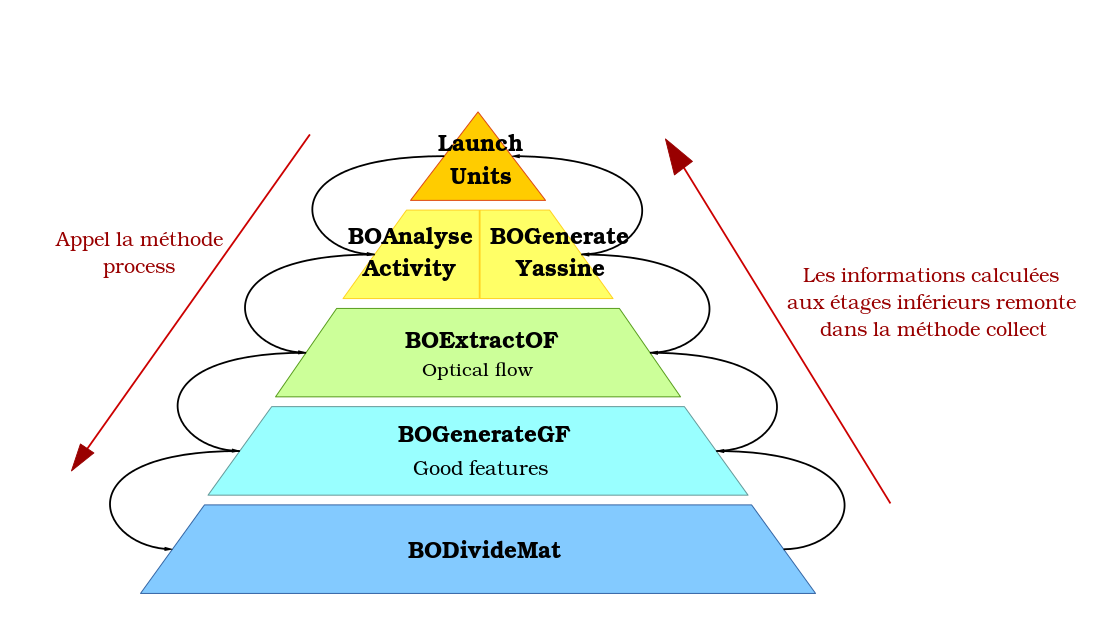
\includegraphics[width=12.5cm]{image/pyramide.png}
  \caption{Processus d'extraction des informations pyramidales sur le flux vidéo}
\end{figure}

Les différentes couches de la pyramide disposent d'une classe métier abstraite. Ces classes 
sont décrites dans la liste suivante :\\

\begin{itemize}
 \item \textbf{BODivideMat} : ces objets métiers découpent une image source en plusieurs images telles que 
 le cadre du visage ou des yeux.
 \item \textbf{BOGenerateGF} : ces objets métiers générent les bonnes particularités (Good Features). 
 À cette étape, le choix des points d'intérêts est effectué, ces points sont dans la zone du visage 
 découpée dans l'étage précédent. Ensuite, les points identiques dans l'image précédente et l'image 
 courante sont conservés.
 \item \textbf{BOExtractOF} : ces objets métiers extraient les flux optiques (Optical Flows) à partir 
 des points générés lors de l'étape précédente. Les flux optiques représentent les mouvements à l'intérieur 
 du visage et doivent être invariants aux mouvements du visage, de la personne ou de la caméra.
 \item \textbf{BOAnalyseActivity et BOGeneteYassine} : ces objets métiers analysent les résultats 
 des flux optiques afin de déterminer les informations sur l'activité à l'intérieur du visage.
 \item \textbf{Lauch Units} : cette unitée n'est pas un objet métier, elle crée les objets métiers des 
 couches inférieures afin d'avoir une exécution du programme qui utilise ces Business Objects.
\end{itemize}
\ \\

Pour notre projet, nous travaillons dans la couche basse de la pyramide. Cette couche divise
les images du flux vidéo en diverses régions d'intérêt telles que la région du visage, puis 
des yeux.

% fusion
\subsection{Détection du visage et des yeux}

L'application est divisée en deux parties. La première recherche le visage grâce à
l'algorithme de Viola et Jones, et la seconde recherche les yeux dans la région délimitée
précédemment.\\

\subsubsection{Détection du visage}
L'algorithme de Viola et Jones\cite{Viola04robustreal-time} est une méthode qui a été créée pour la détection de visages dans une 
image. Cette méthode s'est par la suite généralisée à toutes sortes d'objets. L'algorithme nécessite une 
base de connaissances composée des caractéristiques de l'objet recherché. Elle est utilisée dans un 
apprentissage supervisé, c'est à dire que l'algorithme a besoin de données représentant
l'objet à détecter pour classifier les caractéristiques de celui-ci.\\

Cet algorithme est basé sur des caractéristiques pseudo-Haar qui crée des masques rectangulaires et adjacents
dans différentes zones de l'image. Chaque masque calcule l'intensité des pixels qu'il contient, puis l'algorithme fait
la différence entre les masques blancs et les masque noirs. Cette méthode va permettre de détecter des contours ou des changements de 
texture.\\

\begin{figure}[H]
\center

\includegraphics[width=5cm]{image/pseudo_haar.png}
\caption{Exemple de caractéristiques pseudo-Haar utilisé pour l'algorithme Viola et Jones}
\end{figure}

Pour améliorer les perfomances de leur algorithme, Viola et Jones utilisent la méthode Adaboost. Son
principe est de séléctionner les caractéristiques les plus performantes pour la détection de l'objet grâce à
un calcul de probabilité utilisant l'entropie\footnote{valeur mesurant l'incertitude d'une donnée} des données.\\

Cet algorithme est très efficace pour la détection de visage de l'application, mais nous ne pouvons le mettre
en oeuvre pour la détection des yeux faute de temps. De plus, la base de connaissances nécessaires pour cet 
algorithme doit posséder des miliers d'exemples qu'il nous est impossible de rassembler. C'est pourquoi
un autre algorithme a été utilisé pour la détection des yeux.

\subsubsection{Détection des yeux}
Une fois que la région du visage est reconnue dans le flux vidéo, nous cherchons à détecter les yeux. 
L'algorithme de détection des yeux déjà existant dans l'application permet une détection des yeux 
robuste, mais assez peu précise. Cet algorithme se déroule en plusieurs étapes. D'abord, la région du visage 
retrouvé par la méthode de Viola et Jones est égalisée. Ensuite, elle est scannée de bas en haut afin de
trouver les yeux avant les sourcils. Dans un même temps l'algorithme essaie de retrouver les yeux via la
méthode Means Shift\footnote{technique d'analyse permettant de trouver les maxima dans une fonction de densité}.\\




  \section{Recherche de solution}

\subsection{L'algorithme de Canny}

\subsubsection{Version de base}
%TODO gaetan

\subsubsection{Avec égalisation d'histogramme}
L'égalisation d'histogramme est un procédé qui essaye de placer le même nombre de pixels
sur chaque composante de gris. Ce qui a pour effet d'augmenter le contraste de l'image
et devrait ainsi améliorer les hautes fréquences de l'image, donc les contours. Nous avons
essayé d'appliquer cette méthode sur une image en niveau de gris avant de lancer l'algorithme
de Canny.
%TODO ajout des images

\subsubsection{Avec une moyenne de pixels sur des parties d'image}

\subsubsection{Avec une médiane sur les valeurs de gris des parties d'image}

\subsection{L'algorithme de Gabor}
  \section{Implémentation de la solution}
Plusieurs des solutions que nous avons testées ne nous ont pas permis d'atteindre l'objectif du projet.
Par exemple, nous n'avons pas retenu l'algorithme de Canny, qui malgré plusieurs traitements sur l'algorithme
de base, ne permettait pas de s'abstraire de la luminosité de la vidéo.
Nous allons donc voir en détail les solutions qui ont été utilisées pour atteindre nos objectifs.

\subsection{Solutions utilisées dans l'application}
Lorsque nous analysons une vidéo pour en extraire le centre de l'oeil, nous sommes confrontés à certaines contraintes.
Cependant, la majorité d'entre elles dépendent de la gestion de la couleur de l'image que nous analysons. C'est
pourquoi l'algorithme de Canny n'était pas efficace, car celui-ci était appliqué à une image en dégradé de gris
et donc subissait les effets de la luminosité de la vidéo.\\

Nous avons donc choisi d'utiliser un modèle colorimétrique différent afin d'en extraire une des composantes.
Notre solution utilise le canal de la première chrominance du modèle colorimétrique YCbCr ce qui permet 
de ne plus prendre en compte la couleur de peau et de diminuer l'effet de la luminosité dans l'image que nous traitons.\\

%TODO binarisation

Une fois la binarisation effectuée, nous devons détecter la forme de l'oeil. Pour cela, nous utilisons les blobs, qui nous
permettent non seulement de récupérer des enveloppes convexes présentes dans l'image, mais aussi de déterminer quelle enveloppe
correspond à l'oeil. Pour cela, nous vérifions que l'enveloppe convexe est celle qui est la plus au centre.
Nous calculons ensuite le barycentre de cette forme afin d'obtenir le centre de l'oeil.\\

Cette solution ne gère pas complètement le cas où l'oeil de l'utilisateur est fermé. Dans le cas où notre algorithme
n'arrive pas à calculer le centre de l'oeil, nous récupérons les coordonnées du point qui étaient calculées par la méthode 
de l'équipe. Ainsi, dans le cas où nous ne détectons aucun blob, nous obtenons tout de même un point, sauf si la méthode 
précédente ne fonctionne pas non plus.

\newpage

\subsection{Comparaison des résultats obtenus avec les anciens résultats}
Afin de valider nos travaux, nous pouvons tester notre solution sur des vidéos comportant les points correspondant à 
la vérité terrain. Les vidéos de la base devel ne sont pas annotées, par conséquent nous devons annoter certaines de 
ces vidéos, via un script qui nous permet de relever la vérité terrain image par image. Ensuite, pour comparer les points 
de l'ancienne méthode avec les nôtres, nous calculons la distance entre ces points et la vérité terrain.\\

\begin{figure}[H]
  \centering
  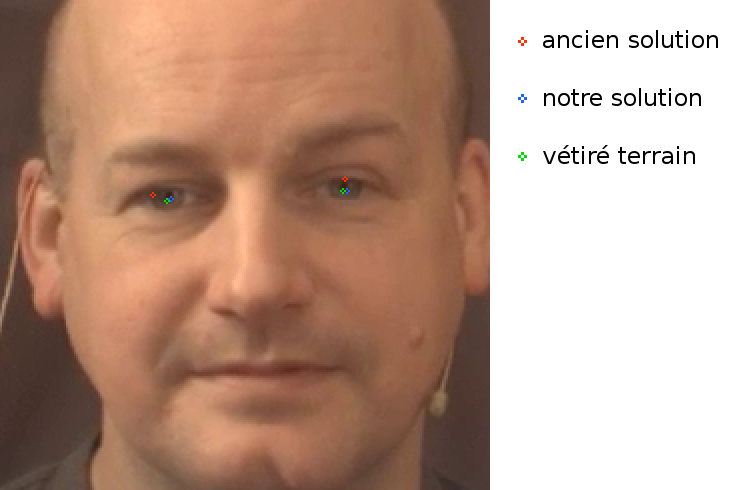
\includegraphics[width=13cm]{image/visage_6points.png}
  \caption{Trois pairs de points pour les yeux}
\end{figure}

\begin{figure}[H]
  \centering
  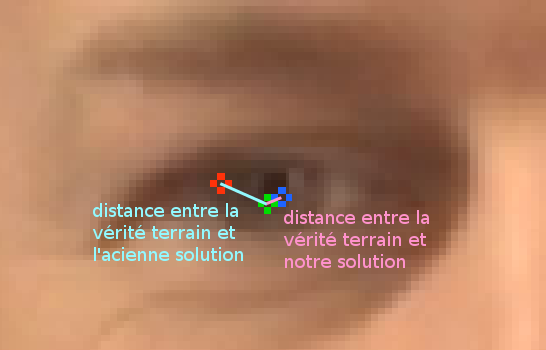
\includegraphics[width=8cm]{image/eye_3points.png}
  \caption{Illustration de la distance avec la vérité terrain}
\end{figure}


Pour avoir des éléments de comparaison, nous faisons la moyenne de ces deux distances pour une vidéo, et nous calculons
le nombre de cas dans lesquels nos points sont plus efficaces. Dans la première vidéo nous obtenons 70\% de points plus précis, et
60\% pour la seconde vidéo.\\

\begin{figure}[H]
  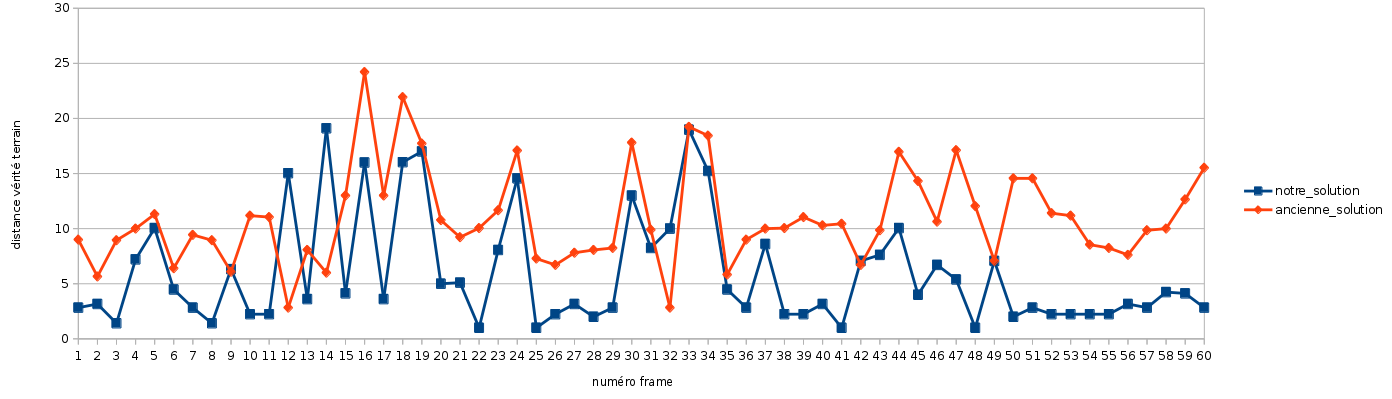
\includegraphics[width=17cm]{resultat/resultat_gauche.png}
  \caption{Comparaison des résultats pour l'oeil gauche}
\end{figure}

\begin{figure}[H]
  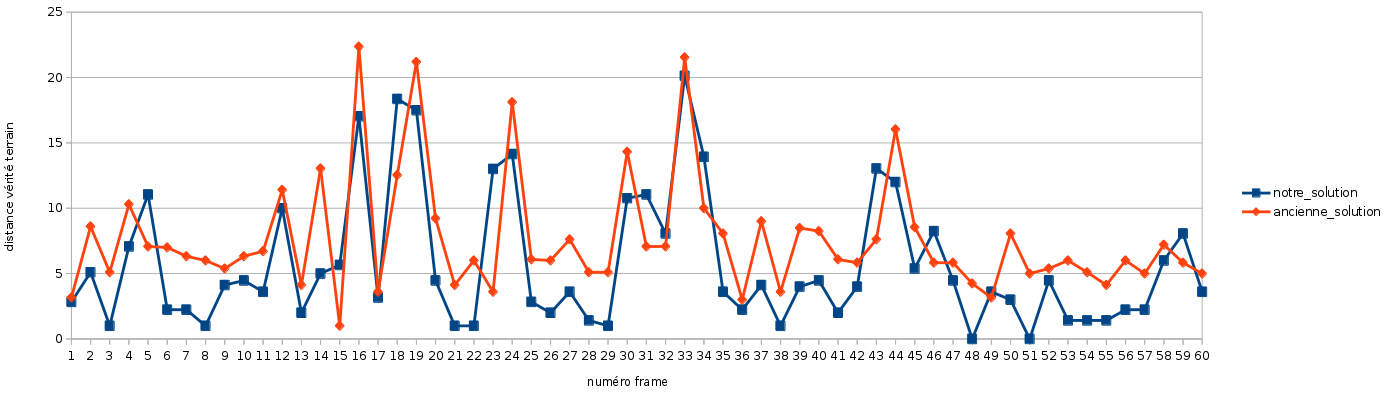
\includegraphics[width=17cm]{resultat/resultat_droit.png}
  \caption{Comparaison des résultats pour l'oeil droit}
\end{figure}

Pour ces résultats, nous avons pris une frame sur vingt-cinq afin d'analyser des mouvements de tête
assez importants. Nous pouvons voir que notre algorithme est plus efficace, en sachant que dans le cas où il ne détecte pas de point, il se repose sur l'ancien
calcul. De plus, nous avons pu constater que la condition que nous posons sur la sélection du blob peut poser problème 
avec le sourcil de la personne quand le blob du sourcil et celui de l'oeil sont à égale distance du centre de la fenêtre.\\

Notre solution améliore donc légèrement la position du centre de l'oeil détecté par l'algorithme de l'équipe FOX. Certaines
situations ne sont pas encore bien gérées dans l'application, mais nous avons pu étudier quelques solutions qui pourraient améliorer
la localisation de l'oeil.

\newpage

\subsection{Améliorations envisageables}
Tous les objectifs n'ont pas été remplis, car la recherche de solution pour l'optimisation du calcul du centre de l'oeil
nous a pris beaucoup de temps à cause des pistes qui n'ont pas abouti. Notre point obtient de meilleurs résultats
que celui utilisé précédement, mais il reste toujours un écart avec la vérité terrain. Il est donc encore possible
d'améliorer notre solution.\\

Le second objectif sur la localisation de l'oeil, lorsque celui-ci est fermé, n'est pas abouti. Notre solution
nous permet de détecter parfois un point dans ce cas. Mais ce qu'il trouve n'est pas le centre de l'oeil mais le
centre des cils qui sont plus visibles lorsque les yeux sont fermés.
%TODO

  \section{Conclusion}
%\addcontentsline{toc}{section}{Conclusion}

\subsection{Bilan sur l'application}

\subsection{Bilan des compétences}

%réussite ou échec du pji

%revenir nous les connaissances qui nous seront util en ivi
\newpage
  \section*{Annexes}
\addcontentsline{toc}{section}{Annexes}



\newpage
  
  % ne pas oublié de citer quelque chose pour que la biblio apparaisse
  \bibliographystyle{plain}
  \bibliography{partie/biblio}
  
\end{document}
